\section{Электростатика}

\begin{ex}
Два маленьких шарика, массы которых $m$ и $M$, заряжены одинаковыми зарядами $q$ и удерживаются на расстоянии $L$ друг от друга. Шарики отпускают, и они начинают разлетаться. Найти скорости шариков после разлета на большое расстояние. Найти скорости шариков после разлета на расстояние $7L$.
\begin{ans}
$v = \sqrt{frac{2Mq^2}{Lm(m+M)}}$, $u = \sqrt{frac{2mq^2}{LM(m+M)}}$
\end{ans}
\end{ex}

%Ижевск
\begin{ex}
Точечный заряд $q$ находится между двумя заземленными проводящими концентрическими сферами 
радиусами $a$ и $b$ на расстоянии $r$ от центра ($a<r<b$). 
Найти полные индуцированные на сферах заряды. Рассмотреть все возможные предельные случаи.
\begin{ans}
$q_a = -q\frac{a(b-r)}{r(b-a)}$, $q_b = -q\frac{b(r-a)}{r(b-a)}$
\end{ans}
\end{ex}

%Ижевск
\begin{ex}
\hspace{0pt} \\
\begin{minipage}{.65\textwidth}
Заряженный металлический шар радиуса $R$ разрезан на две части по плоскости, отстоящей от центра на расстояние $h$. 
Найти силу, с которой отталкиваются эти части. Исходный заряд шара~$Q$.
\end{minipage}
\begin{minipage}{.35\textwidth}
\centering
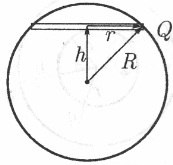
\includegraphics[width = 0.55 \textwidth]{1003ElectrostaticsBall.jpg}
\end{minipage}
\begin{ans}
$F = \frac{Q^2 \pi (R^2-h^2)}{2 \varepsilon_0 {(4 \pi R^2)}^2}$
\end{ans}
\end{ex}

%Ижевск
\begin{ex}
\hspace{0pt} \\
\begin{minipage}{.65\textwidth}
Грани правильного тетраэдра со стороной $a$ равномерно заряжены с поверхностной плотностью заряда $\sigma$. 
В центр тетраэдра помещен точечный заряд $q$. Найти силу, с которой точечный заряд действует на одну из граней тетраэдра.
\end{minipage}
\begin{minipage}{.35\textwidth}
\centering
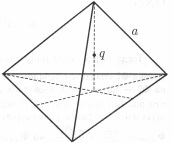
\includegraphics[width = 0.65 \textwidth]{1004ElectrostaticsTetrahedron.jpg}
\end{minipage}
\begin{ans}
$F = \frac{\sigma^2 \sqrt{3}a^2}{8\varepsilon_0}$
\end{ans}
\end{ex}

%Ижевск
\begin{ex}
\hspace{0pt} \\
\begin{minipage}{.65\textwidth}
Две большие проводящие пластины $1$ и $2$ расположены на расстоянии $d$ друг от друга, 
а между ними на расстоянии $х$ от пластины $1$ находится проводящая пластина с зарядом $q$. 
Крайние пластины соединены проводником и имеют заряд $-q$. 
Какой заряд пройдет по проводнику, соединяющему крайние пластины, если пластину с зарядом $q$ переместить из положения $x$ в положение с координатой~$x_1$.
\end{minipage}
\begin{minipage}{.35\textwidth}
\centering
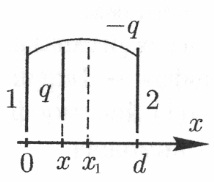
\includegraphics[width = 0.9 \textwidth]{1005ElectrostaticsTwoPlates.jpg}
\end{minipage}
\begin{ans}
$\mid\Delta q \mid = \mid q \frac{x-x_1}{d}$
\end{ans}
\end{ex}

\begin{ex}
(2017) В вакууме относительно некоторой ИСО покоится однородное тонкое кольцо радиуса $R$, массой $3m$ и равномерно распределенным зарядом $q$. Какую минимальную скорость в этой ИСО должна иметь частица массой $m$ и зарядом равным по знаку и величине заряду кольца, чтобы, двигаясь вдоль оси кольца с очень большого расстояния, достичь его центра? Рассмотрите два случая: а) кольцо закреплено; б) кольцо свободное.
\begin{ans}
$v_{\min} = q\sqrt{\frac{2k}{mR}}$, $v_{\min 2} = q\sqrt{\frac{8k}{3mR}}$, 
\end{ans}
\end{ex}

\section{Конденсаторы}

\begin{ex}
\hspace{0pt} \\
\begin{minipage}{.65\textwidth}
В электрической схеме, изображенной на рисунке, в начальный момент времени ключ $K$ разомкнут, конденсатор не заряжен. 
Параметры схемы указаны на рисунке. Определите начальные токи через резисторы и через батарею сразу после замыкания.
\end{minipage}
\begin{minipage}{.35\textwidth}
\centering
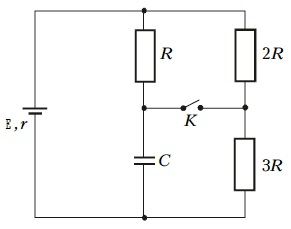
\includegraphics[width = 0.9 \textwidth]{1001Condensers.jpg}
\end{minipage}
\begin{ans}
$I_{01} = \frac{3 \mathcal{E}}{3r+2R}$, $I_{02} = \frac{\mathcal{E}}{3r+2R}$
\end{ans}
\end{ex}

%Ижевск
\begin{ex}
\hspace{0pt} \\
\begin{minipage}{.65\textwidth}
Батарея с ЭДС, равной $\mathcal{E}$, конденсаторы емкостями $C_1$ и $C_2$ и резистор сопротивлением $R$ соединены так, как показано на рисунке. 
Найдите количество теплоты $Q$, выделяющееся на резисторе после переключения ключа~$K$.
\end{minipage}
\begin{minipage}{.35\textwidth}
\centering
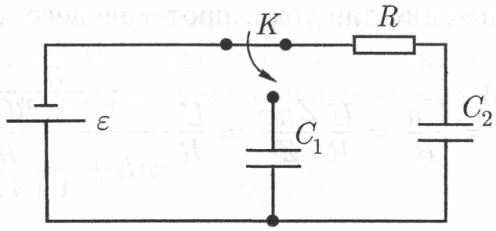
\includegraphics[width = 0.9 \textwidth]{1002Condensers.jpg}
\end{minipage}
\begin{ans}
$Q=\frac{C_1C_2 \mathcal{E}^2}{2(C_1+C_2)}$
\end{ans}
\end{ex}

\begin{ex} 
По какому закону изменяется ток через изначально незаряженный конденсатор емкости $C$, подключенный к источнику тока $U$ через сопротивление~$R$?
\begin{ans}
$I = \frac{U}{R} e^{-t/RC}$
\end{ans}
\end{ex}

\begin{ex} 
\hspace{0pt} \\
\begin{minipage}{.65\textwidth}
Две батареи включены в схему, изображенную на рисунке (сопротивления всех резисторов равны $R$). 
Первоначально конденсаторы не заряжены, а ключи разомкнуты. Ключи одновременно замыкают. 
1) Найти начальный ток через резистор $R_1$. 2) Какое количество теплоты выделится во всей схеме после замыкания ключей?
\end{minipage}
\begin{minipage}{.35\textwidth}
\centering
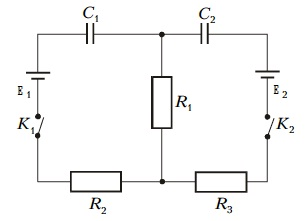
\includegraphics[width = 0.9 \textwidth]{1005Condensers.jpg}
\end{minipage}
\begin{ans}
1) $I_1=\frac{\mathcal{E}_1 + \mathcal{E}_2}{3R}$; 2) $Q=(C_1 \mathcal{E}_1^2 + C_2 \mathcal{E}_2^2/2)$
\end{ans}
\end{ex}

\begin{ex} 
\hspace{0pt} \\
\begin{minipage}{.65\textwidth}
В схеме на рисунке ключи разомкнуты, а конденсаторы не заряжены. Ключ $K_1$ замыкают, оставляя ключ $K_2$ разомкнутым. 
1) Какие напряжения установятся на конденсаторах? 2) Какой заряд протечет через ключ $K_2$ при замыкании?
\end{minipage}
\begin{minipage}{.35\textwidth}
\centering
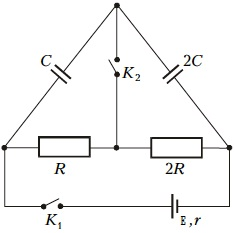
\includegraphics[width = 0.75 \textwidth]{1006Condensers.jpg}
\end{minipage}
\begin{ans}
1) $U_1 = \frac{2R \mathcal{E}}{r+3R}$, $U_2 = \frac{R \mathcal{E}}{r+3R}$; 2) $Q=\frac{3RC\mathcal{E}}{r+3R}$
\end{ans}
\end{ex}